\section{Légendes et normes communes}

Les cinq politiques de cohérences gérées par le simulateur sont MSI, MESI, MOSI, MESIF et MOESI. Ces politiques servent à décrire l'état d'une ligne dans un cache, et ainsi pouvoir effetuer certaines actions en cas d'évènement impliquant la ligne : par exemple si elle est lue. Les évènements suivants sont possibles :
\begin{itemize}
\item{\verb!i_read! : le cache courant lit la ligne}
\item{\verb!a_read! : un autre cache du même niveau lit la ligne}
\item{\verb!i_write! : le cache courant modifie la ligne}
\item{\verb!a_write! : un autre cache du même niveau modifie la ligne}
\item{\verb!i_del! : le cache courant supprime la ligne}
\item{\verb!a_del! : un autre cache du même niveau supprime la ligne}\\
\end{itemize}
Ces évènements correspondent aux transitions entre les états possibles d'une ligne. Ces états possibles sont : M, E, S, O, I, F, présents ou non suivant la politique étudiée.

\paragraph{}
Lors d'une transition, une action peut-être effectuée, ce qui nous intéresse dans le cadre de la simulation sont certaines statistiques. Les politiques de cohérence ont pour charge le compte des \verb!COHERENCE_BROADCAST!, \verb!COHERENCE_EVINCTION! et \verb!WRITE_BACK!. Ce sont en effet les seules statistiques implémentées propres à la cohérence. L'autre statistique gérée par ces politiques, mais qui n'est pas implémentée, est la bande-passante d'un niveau de cache. 

\paragraph{}
Certaines transitions sont conditionnelles : elles ne se produisent qu'en fonction de l'utilisation de la ligne par les autres caches du même niveau. Elles sont ici représentées par une égalité ou inégalité, entre crochets.

\paragraph{}
Notons que tous les automates sont déterministes, toutes les transitions qui ne sont pas représentées sont en réalité des boucles, ne donnant lieu à aucune action.


\section{Représentations des automates}
\label{aut}

\begin{figure}[!h]
\begin{center}
   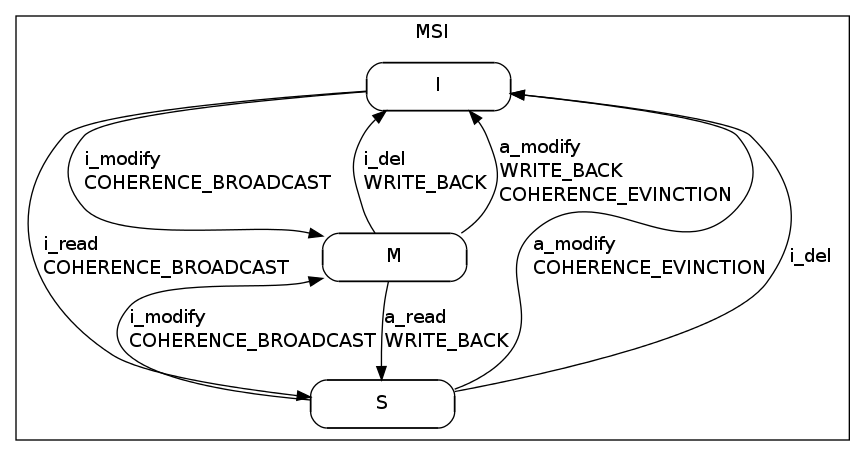
\includegraphics[scale=0.45]{images/MSI_simple.png}
   \caption{\label{img:state_msi} Automate des états MSI}
\end{center}
\end{figure}


\begin{figure}[!h]
\begin{center}
   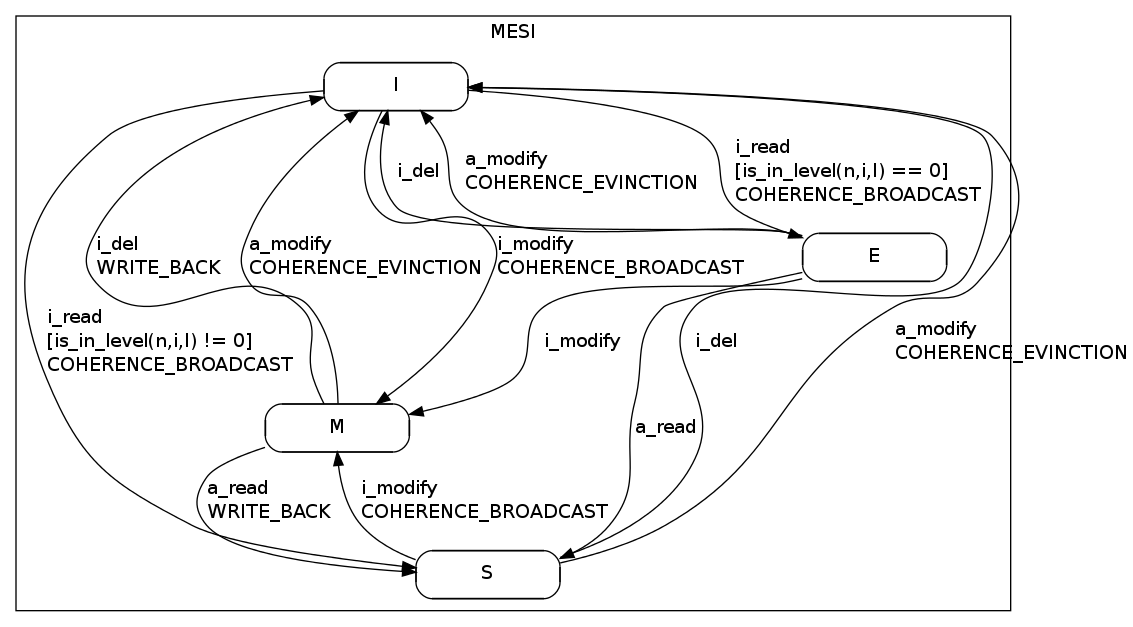
\includegraphics[scale=0.4]{images/MESI_simple.png}
   \caption{\label{img:state_mesi} Automate des états MESI}
\end{center}
\end{figure}


\begin{figure}[!h]
\begin{center}
   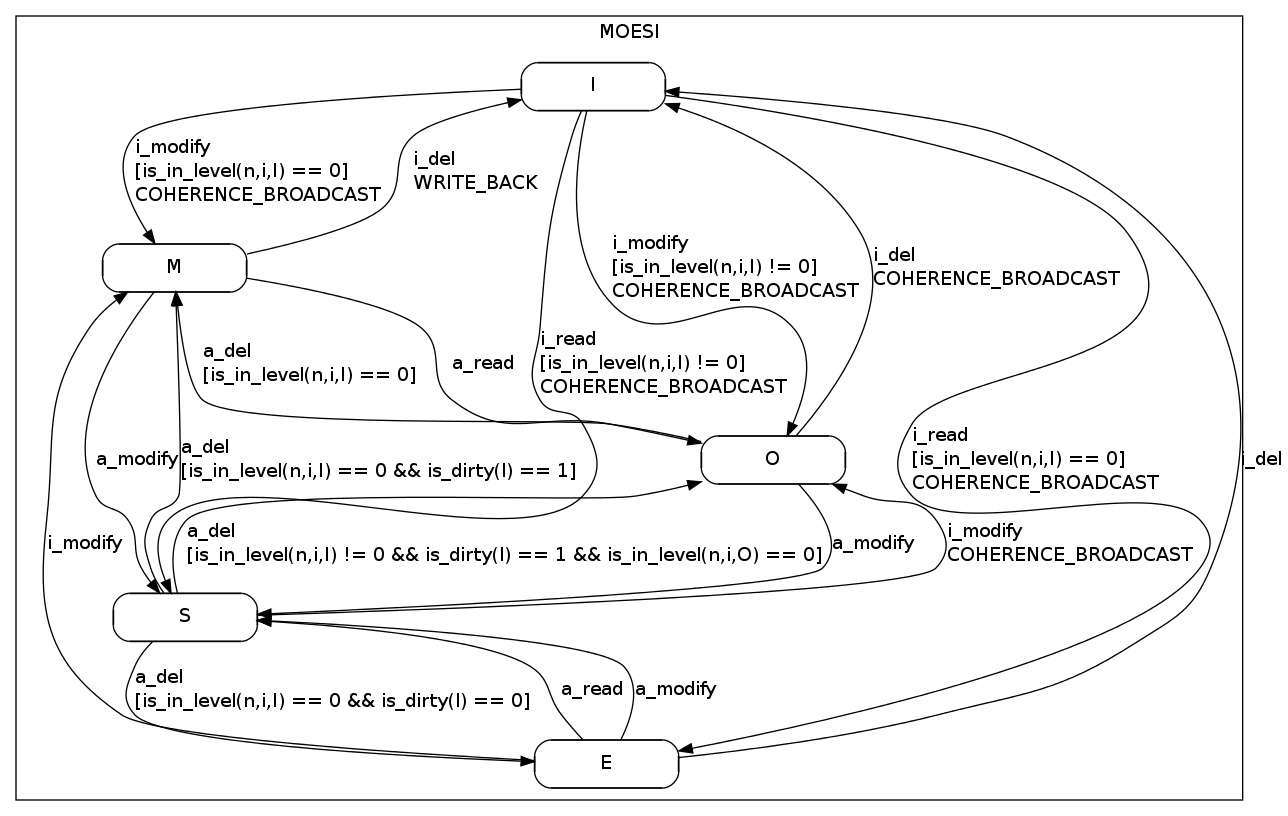
\includegraphics[scale=0.35]{images/MOESI_simple.png}
   \caption{\label{img:state_moesi} Automate des états MOESI}
\end{center}
\end{figure}


\begin{figure}[!h]
\begin{center}
   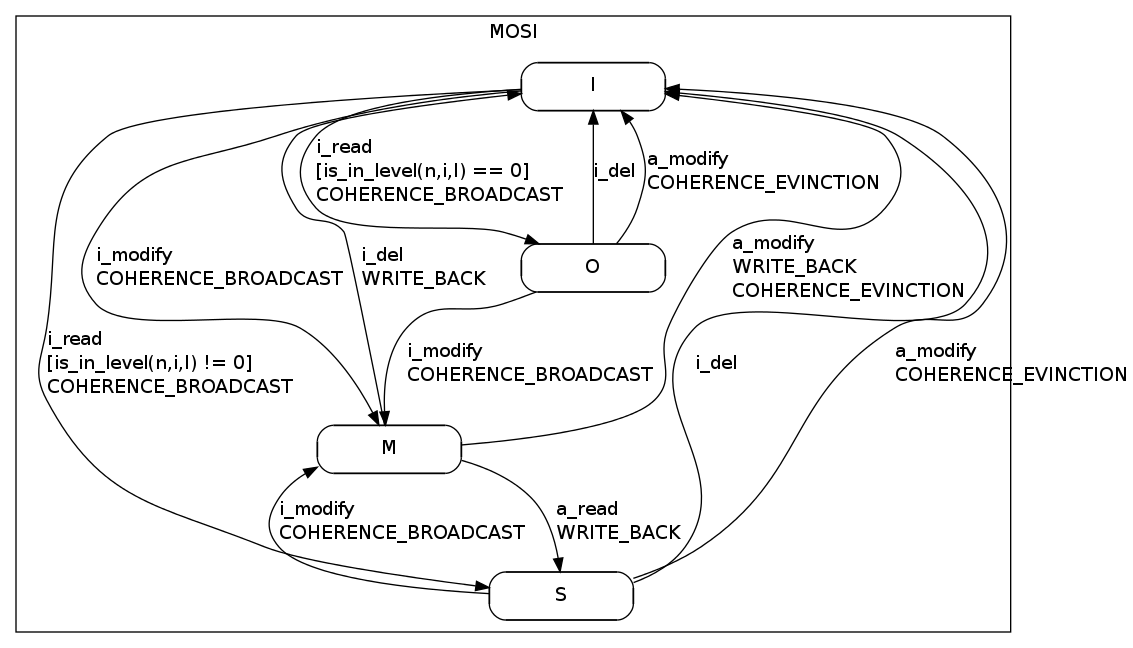
\includegraphics[scale=0.4]{images/MOSI_simple.png}
   \caption{\label{img:state_mosi} Automate des états MOSI}
\end{center}
\end{figure}


\begin{figure}[!h]
\begin{center}
   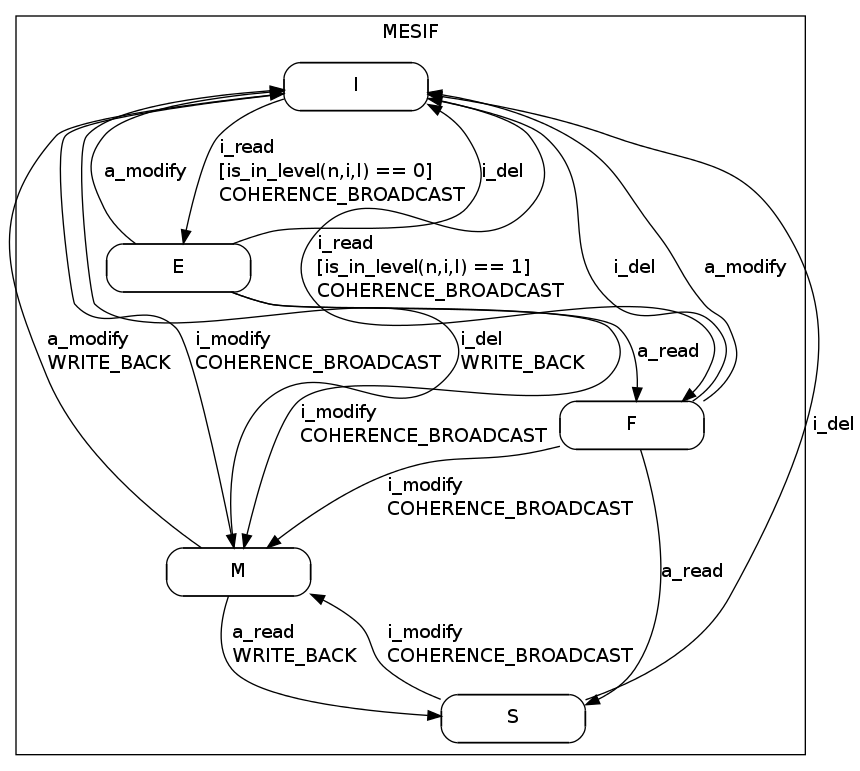
\includegraphics[scale=0.5]{images/MESIF_simple.png}
   \caption{\label{img:state_mesif} Automate des états MESIF}
\end{center}
\end{figure}


